\section{1174008 - Arjun Yuda Firwanda}

\subsection{Teori}
\begin{enumerate}

        \item Jelaskan kenapa file teks harus di lakukan tokenizer
Untuk memudahkan mesin memahami maksud dari apa yang kita inginkan dalam machine learning, kata pada teks disebut token, dan proses vektorisasi dari bentuk kata ke dalam token tersebut disebut tokenizer dan tokenizer akan merubah sebuah teks menjadi simbol, kata, ataupun biner dan bentuk lainnya kedalam token. 

	\begin{figure}[H]
            	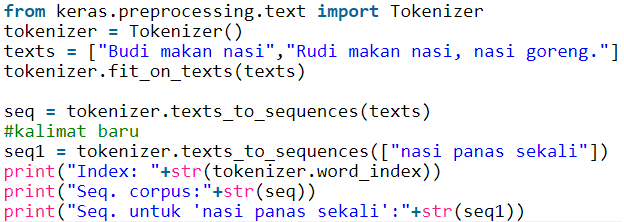
\includegraphics[width=4cm]{figures/1174008/7/teori1.PNG}
           	 \centering
           	 \caption{Tokenizer}
        	\end{figure}

        \item Jelaskan konsep dasar K Fold Cross Validation pada dataset komentar Youtube
Konsep dasar StartifiedKFold berisikan presentasi sampel untuk setiap kelas. Dimana dalam ilustrasi ini sampel dibagi menjadi 5 dalam setiap class nya. Kemudian sampel tadi akan dimasukan kedalam class dari dataset youtube.

	\begin{figure}[H]
		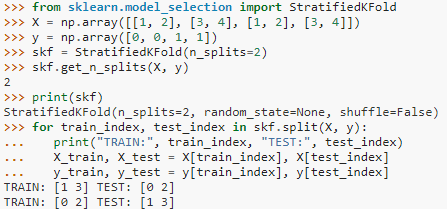
\includegraphics[width=4cm]{figures/1174008/7/teori2.PNG}
            	\centering
           	 \caption{K Fold Coss Validation}
       	 \end{figure}

        \item Jelaskan apa maksudnya kode program for train, test in splits
Maksudnya yaitu untuk menguji apakah setiap data pada dataset sudah di split dan tidak terjadi penumpukan. Yang dimana maksudnya di setiap class tidak akan muncul id yang sama. Ilustrasinya misalkan kita memiliki 4 baju dengan model yang berbeda. Kemudian kita bagikan kedua anak, tentunya setiap anak yang menerima baju tidak memiliki baju yang sama modelnya.

        \item Jelaskan apa maksudnya kode program train content 
Maksudnya yaitu mengambil data pada kolom atau index CONTENT yang merupakan bagian dari train\_idx dan test\_idx. Ilustrasinya, ketika data telah diubah menjadi train dan test maka kita dapat memilihnya untuk ditampilkan pada kolom yang diinginkan.

        \item Jelaskan apa maksud dari fungsi tokenizer 
Dimana variabel tokenizer akan melakukan vektorisasi kata menggunakan fungsi Tokenizer yang dimana jumlah kata yang ingin diubah kedalam bentuk token adalah 2000 kata. Dan untuk \emph{tokenizer.fit\_on\_texts(train\_content)} maksudnya kita akan melakukan fit tokenizer hanya untuk dat trainnya saja tidak dengan data test nya untuk kolom CONTENT.

        \item Jelaskan apa maksud dari fungsi d train inputs = tokenizer.texts to matrix
Maksudnya yaitu untuk variabel d\_train\_inputs akan melakukan tokenizer dari bentuk teks ke matrix dari data train\_content dengan mode matriksnya yaitu tfidf begitu juga dengan variabel d\_test\_inputs untuk data test. Berikut gambar ilustrasinya

	\begin{figure}[H]
		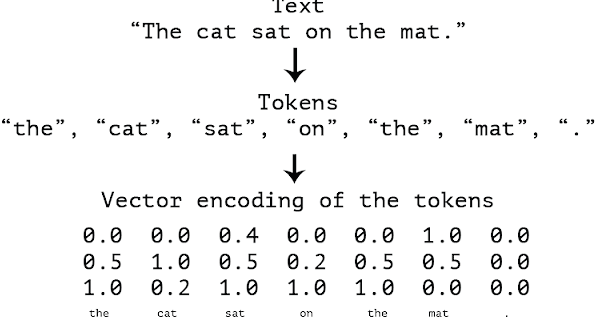
\includegraphics[width=4cm]{figures/1174008/7/teori3.PNG}
            	\centering
           	 \caption{tokenizer.texts to matrix}
       	 \end{figure}

        \item Jelaskan apa maksud dari fungsi d train inputs = d train inputs/np.amax
Fungsi tersebut akan membagi matrix tfidf tadi dengan amax yaitu mengembalikan maksimum array atau maksimum sepanjang sumbu. Yang hasilnya akan dimasukan kedalam variabel d\_train\_inputs untuk data train dan d\_test\_inputs untuk data test dengan nominal absolut atau tanpa ada bilangan negatif dan koma.

	\begin{figure}[H]
		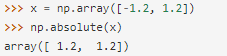
\includegraphics[width=4cm]{figures/1174008/7/teori4.PNG}
            	\centering
           	 \caption{d train inputs/np.amax}
       	 \end{figure}

        \item Jelaskan apa maksud fungsi dari d train outputs = np utils.to categorical
Dalam variabel d\_train\_output dan d\_test\_outputs akan dilakukan one hot encoding, dimana np\_utilsakan mengubah vektor dengan bentuk integer ke matriks kelas biner untuk kolom CLASS dimana nantinya hanya akan ada dua pilihan yaitu 1 atau 0. 1 untuk spam 0 untuk non spam atau sebaliknya.

	\begin{figure}[H]
		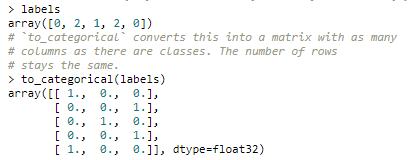
\includegraphics[width=4cm]{figures/1174008/7/teori5.PNG}
            	\centering
           	 \caption{np utils.to categorical}
       	 \end{figure}

        \item Jelaskan apa maksud dari fungsi di listing 7.2. Gambarkan ilustrasi Neural Network nya dari model kode tersebut.
Melakukan pemodelan Sequential. Layer pertama dense dari 512 neuron untuk inputan dengan inputan tadi yang sudah dijadikan matriks sebanyak 2000. Activationnya menggunakan fungsi relu yaitu jika ada inputan dengan nilai maksimum maka inputan itu yang akan terpilih. Dropout ini untuk melakukan pembobotan, dimana pembobotan hanya dilakukan 50\% saja agar tidak terjadi penumpukan data dari dense inputan tadi. Dense 2 mengkategorikan 2 neuron untuk output nya yaitu 1 dan 0. Untuk dense diatas aktivasinya menggunakan fungsi Softmax.

	\begin{figure}[H]
		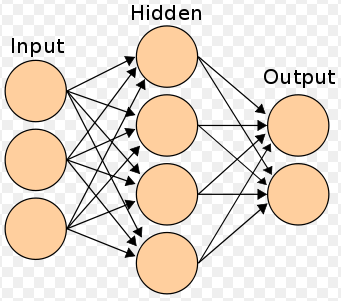
\includegraphics[width=4cm]{figures/1174008/7/teori6.PNG}
            	\centering
           	 \caption{fungsi di listing 7.2}
       	 \end{figure}

        \item Jelaskan apa maksud dari fungsi di listing 7.3 dengan parameter tersebut.
Melakukan peng compile-an dari model Sequential tadi dengan Loss yandengang merupakan fungsi optimisasi skor  menggunakan categorical\_crossentropy , dan menggunakan algoritma adam sebagai optimizer. Adam yaitu algoritma pengoptimalan yang dapat digunakan sebagai ganti dari prosedur penurunan gradien stokastik klasik untuk memperbarui bobot jaringan yang berulang berdasarkan data training.Dengan metrik yaitu fungsi yang digunakan untuk menilai kinerja mode Anda disini menggunakan fungsi accuracy.

        \item Jelaskan apa itu Deep Learning
Deep Learning merupakan subbidang machine learning yang berkaitan dengan algoritma yang terinspirasi oleh struktur dan fungsi otak yang disebut jaringan saraf tiruan atau Artificial Neural Networks. Jaringan saraf tiruan, algoritma yang terinspirasi oleh otak manusia, belajar dari sejumlah besar data. Demikian pula dengan bagaimana kita belajar dari pengalaman, algoritma pembelajaran yang mendalam akan melakukan tugas berulang kali, setiap kali sedikit mengubahnya untuk meningkatkan hasilnya.

        \item Jelaskan apa itu Deep Neural Network, dan apa bedanya dengan Deep Learning
Deep Neural Network merupakan jaringan syaraf tiruan (JST) dengan beberapa lapisan antara lapisan input dan output. DNN menemukan manipulasi matematis yang benar untuk mengubah input menjadi output, apakah itu hubungan linear atau hubungan non-linear. Merupakan jaringan syaraf dengan tingkat kompleksitas tertentu, jaringan syaraf dengan lebih dari dua lapisan. Deep Neural Network menggunakan pemodelan matematika yang canggih untuk memproses data dengan cara yang kompleks.

DNN hanya terdiri dari dua laipsan yaitu input dan output, sedangkan dalam Deep learning kita dapat mendefiniskan layer sebanyak yang kita inginkan atau butuhkan.

        \item Jelaskan dengan ilustrasi gambar buatan sendir

Deep Learning merupakan subbidang machine learning yang berkaitan dengan algoritma yang terinspirasi oleh struktur dan fungsi otak yang disebut jaringan saraf tiruan atau Artificial Neural Networks. Jaringan saraf tiruan, algoritma yang terinspirasi oleh otak manusia, belajar dari sejumlah besar data. Demikian pula dengan bagaimana kita belajar dari pengalaman, algoritma pembelajaran yang mendalam akan melakukan tugas berulang kali, setiap kali sedikit mengubahnya untuk meningkatkan hasilnya.

	\item Terdapat data seperti berikut 
		\begin{figure}[ht]
			\centering
			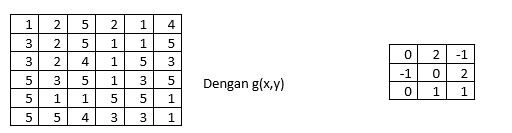
\includegraphics[width=2cm]{figures/1174008/7/teori7.PNG}
			\caption{Algoritma Konvulusi}
			\label{Teori}
		\end{figure}
	
	\item Kemudian hitung konvolusi untuk setiap matriksnya seperti berikut :
	
	\item pertama
		\begin{figure}[ht]
			\centering
			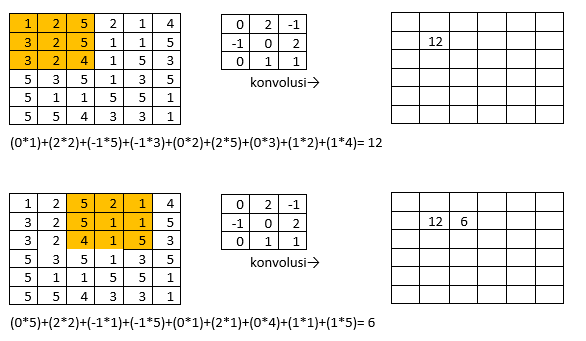
\includegraphics[width=2cm]{figures/1174008/7/teori8.PNG}
			\caption{Algoritma Konvulusi}
			\label{Teori}
		\end{figure}

	\item Kedua
		\begin{figure}[ht]
			\centering
			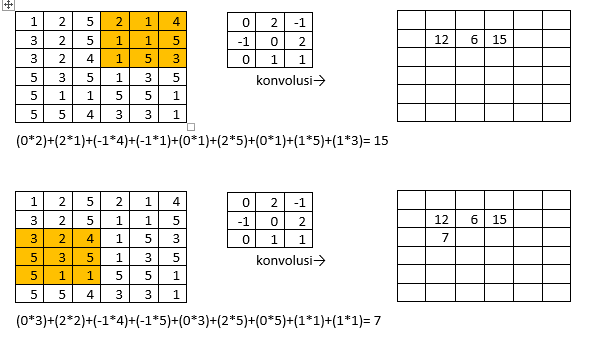
\includegraphics[width=2cm]{figures/1174008/7/teori9.PNG}
			\caption{Algoritma Konvulusi}
			\label{Teori}
		\end{figure}

	\item Ketiga
		\begin{figure}[ht]
			\centering
			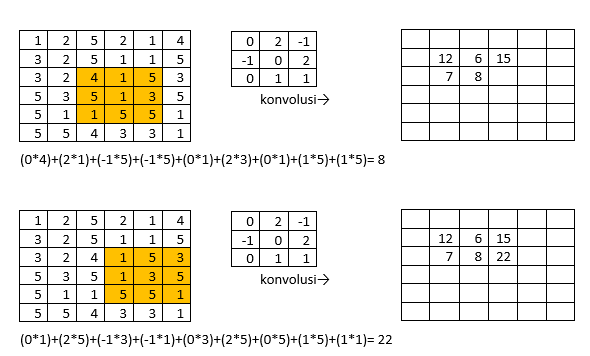
\includegraphics[width=2cm]{figures/1174008/7/teori10.PNG}
			\caption{Algoritma Konvulusi}
			\label{Teori}
		\end{figure}

	\item Keempat
		\begin{figure}[ht]
			\centering
			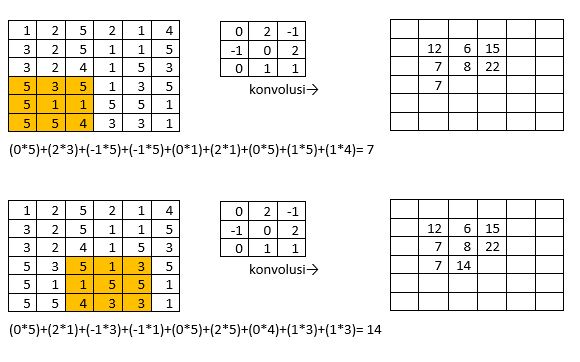
\includegraphics[width=2cm]{figures/1174008/7/teori11.PNG}
			\caption{Algoritma Konvulusi}
			\label{Teori}
		\end{figure}

	\item Kelima
		\begin{figure}[ht]
			\centering
			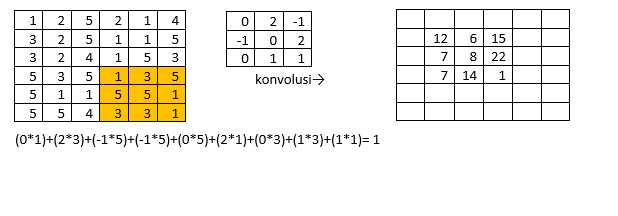
\includegraphics[width=2cm]{figures/1174008/7/teori12.PNG}
			\caption{Algoritma Konvulusi}
			\label{Teori}
		\end{figure}

	\item Didapatkan hasil akhir nilai konvolusi dan juga max poolingnya seperti berikut
		\begin{figure}[ht]
			\centering
			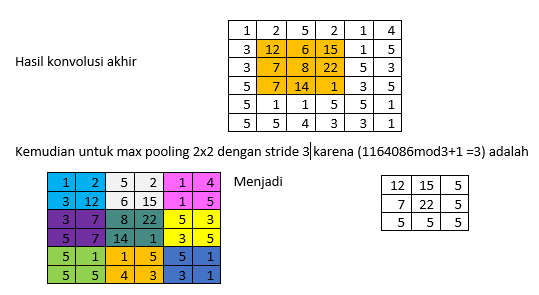
\includegraphics[width=2cm]{figures/1174008/7/teori13.PNG}
			\caption{Algoritma Konvulusi}
			\label{Teori}
		\end{figure}

\end{enumerate}

\subsection{Praktek}
\begin{enumerate}

\item Jelaskan kode program pada blok. Jelaskan arti dari setiap baris kode yang dibuat(harus beda dengan teman sekelas) dan hasil luarannya dari komputer sendiri.

Pertama kita akan mengimpor librari csv. Dimana dari librai PIL atau Pillow atau Python Imaging Library akan diimpor modul Image yang di inisiasikan sebagain pil\_image. Modul Image menyediakan kelas dengan nama yang sama yang digunakan untuk mewakili gambar PIL. Modul ini juga menyediakan sejumlah fungsi pabrik, termasuk fungsi untuk memuat image dari file, dan untuk membuat image baru. Mengimpor librari image dari keras .Yang menghasilkan kumpulan data gambar tensor dengan augmentasi data waktu nyata. Data akan diulang (dalam batch). 

\lstinputlisting[firstline=1, lastline=4]{src/1174008/7/1.py}

	\begin{figure}[H]
		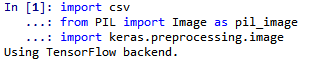
\includegraphics[width=4cm]{figures/1174008/7/praktik1.PNG}
            	\centering
           	 \caption{Praktik1}
       	 \end{figure}

\item Jelaskan kode program pada blok. Jelaskan arti dari setiap baris kode yang dibuat(harus beda dengan teman sekelas) dan hasil luarannya dari komputer sendiri.

Variabel imgs berisikan array kosong. Variabel classes berisikan array kosong. Membuka file csv dari Folder HSYv2 dengan nama file hasy-data-labels.csv sebagai csvfile. Variabel csvreader akan menggunakan fungsi reader pada library csv untuk membaca file csv tadi yang disimpan di csvfile. Dimana variabel i dimuali dari nol. Untuk setiap baris pada  csvreader. Jika i lebih besar dari 0. Jadi itu akan mengambil contoh Gambar PIL dan mengubahnya menjadi array numpy dengan mengambil data dari HSYv2 dan dimulai dari baris ke nol. Hasil dari variabel img akan dibagi dengan 255.0. Append akan membuat list array baru untuk baris 0 baris 2 pada img. Menyimpan setiap class nya  pada baris 2. Penambahan i sebanyak 1.

\lstinputlisting[firstline=1, lastline=15]{src/1174008/7/2.py}

	\begin{figure}[H]
		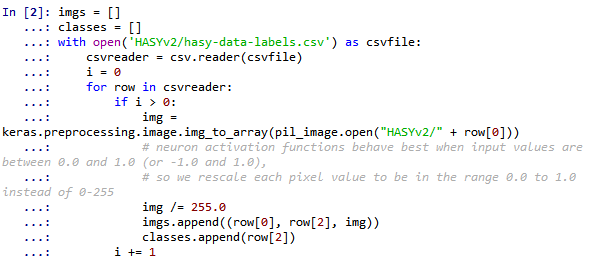
\includegraphics[width=4cm]{figures/1174008/7/praktik2.PNG}
            	\centering
           	 \caption{Praktik2}
       	 \end{figure}

\item Jelaskan kode program pada blok. Jelaskan arti dari setiap baris kode yang dibuat(harus beda dengan teman sekelas) dan hasil luarannya dari komputer sendiri.

Import library Random dari Python. Melakukan pengacakan untuk imgs dengan Metode Shuffle  untuk mengocok urutan di tempat. yaitu, mengubah posisi item dalam daftar. Membagi data dari imgs dengan cara mengalikan 80\% dengan jumlah data dari imgs. Untuk data train mengambil hasil dari perhitungan sebelumnya. Untuk data test mengambil sisa dari jumlah yang telah dijadikan data train

\lstinputlisting[firstline=1, lastline=6]{src/1174008/7/3.py}

	\begin{figure}[H]
		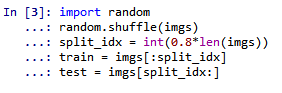
\includegraphics[width=4cm]{figures/1174008/7/praktik3.PNG}
            	\centering
           	 \caption{Praktik3}
       	 \end{figure}


\item Jelaskan kode program pada blok. Jelaskan arti dari setiap baris kode yang dibuat(harus beda dengan teman sekelas) dan hasil luarannya dari komputer sendiri.

Impotr library Numpy yang di inisiasikan sebagai np. Variabel train\_input mengubah input menjadi sebuah array yang diambil dari baris 2, data train. Variabel test\_input mengubah input menjadi sebuah array yang diambil dari baris 2, data test. Variabel train\_output mengubah input menjadi sebuah array yang diambil dari baris 1, data train. Variabel train\_output mengubah input menjadi sebuah array yang diambil dari baris 1, data test.

\lstinputlisting[firstline=1, lastline=9]{src/1174008/7/4.py}

	\begin{figure}[H]
		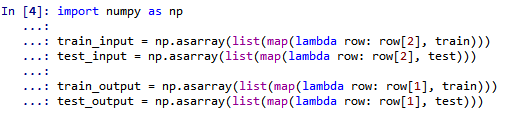
\includegraphics[width=4cm]{figures/1174008/7/praktik4.PNG}
            	\centering
           	 \caption{Praktik4}
       	 \end{figure}


\item Jelaskan kode program pada blok. Jelaskan arti dari setiap baris kode yang dibuat(harus beda dengan teman sekelas) dan hasil luarannya dari komputer sendiri.

Impor Fungsi LabelEncoder dan Impor Fungsi OneHotEncoder

\lstinputlisting[firstline=1, lastline=3]{src/1174008/7/5.py}

	\begin{figure}[H]
		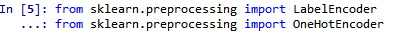
\includegraphics[width=4cm]{figures/1174008/7/praktik5.PNG}
            	\centering
           	 \caption{Praktik5}
       	 \end{figure}

\item Jelaskan kode program pada blok. Jelaskan arti dari setiap baris kode yang dibuat(harus beda dengan teman sekelas) dan hasil luarannya dari komputer sendiri.

Variabel label\_encoder akan memanggil fungsi LabelEncoder tadi. Variabel integer\_encoded akan menggunakan labelencoder untuk melakukan fit pada classes agar berubah datanya menjadi integer.

\lstinputlisting[firstline=1, lastline=5]{src/1174008/7/6.py}

	\begin{figure}[H]
		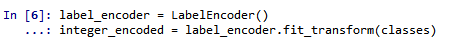
\includegraphics[width=4cm]{figures/1174008/7/praktik6.PNG}
            	\centering
           	 \caption{Praktik6}
       	 \end{figure}

\item Jelaskan kode program pada blok. Jelaskan arti dari setiap baris kode yang dibuat(harus beda dengan teman sekelas) dan hasil luarannya dari komputer sendiri.

Variabel onehot\_encoder akan memanggil fungsi OneHotEncoder dimana tidak berisikan matriks sparse. Pada variabel integer\_encoded akan diubah bentuknya dimana setiap nilai integer akan direpresentasikan sebagai vektor binari dengan nilai 0 kecuali index dari integer tersebut ditandai dengan 1. Melakukan fit untuk one hot encoder kedalam integer\_encoder.

\lstinputlisting[firstline=1, lastline=4]{src/1174008/7/7.py}

	\begin{figure}[H]
		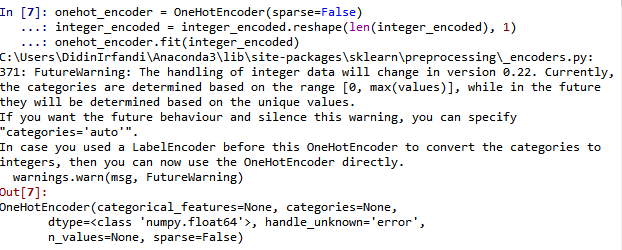
\includegraphics[width=4cm]{figures/1174008/7/praktik7.PNG}
            	\centering
           	 \caption{Praktik7}
       	 \end{figure}

\item Jelaskan kode program pada blok. Jelaskan arti dari setiap baris kode yang dibuat(harus beda dengan teman sekelas) dan hasil luarannya dari komputer sendiri.

Variabel train\_output\_int  akan mengubah data dari train\_output menjadi LabeEncoder. Dimana pada train\_output setelah diubah labelnya menjadi integer dilakukan one hot encoding diambil dari train\_output\_int dan menggunakan .reshape untuk memberikan bentuk baru ke array tanpa mengubah datanya dengan keterangan jika index dari integer tersebut ditandai dengan 1 dan sisanya yang bukan nol. Variabel test\_output\_int  akan mengubah data dari test\_output menjadi LabeEncoder. Dimana pada train\_output setelah diubah labelnya menjadi integer dilakukan one hot encoding diambil dari test\_output\_int dan menggunakan .reshape untuk memberikan bentuk baru ke array tanpa mengubah datanya dengan keterangan jika index dari integer tersebut ditandai dengan 1 dan sisanya yang bukan nol. Variabel num\_classes akan menampilakn jumlah data dari classes yang telah dilakukan label encoder. Menampilkan tulisan "Number of classes : \%d dmana mengembalikan nilai integer dari num\_classes.

\lstinputlisting[firstline=1, lastline=8]{src/1174008/7/8.py}

	\begin{figure}[H]
		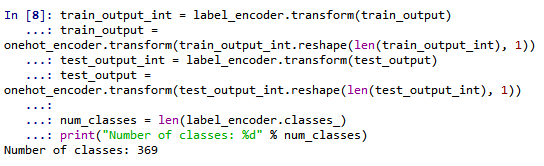
\includegraphics[width=4cm]{figures/1174008/7/praktik8.PNG}
            	\centering
           	 \caption{Praktik8}
       	 \end{figure}

\item Jelaskan kode program pada blok. Jelaskan arti dari setiap baris kode yang dibuat(harus beda dengan teman sekelas) dan hasil luarannya dari komputer sendiri.

Import Sequential dari model pada librari Keras. Import Dense, Dropout, Flatten dari modul Layers pada librari Keras. Impotr Conv2D, MaxPooling2D dari modul Layers pada librari Keras.

\lstinputlisting[firstline=1, lastline=5]{src/1174008/7/9.py}

	\begin{figure}[H]
		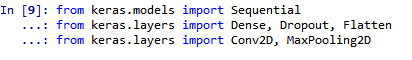
\includegraphics[width=4cm]{figures/1174008/7/praktik9.PNG}
            	\centering
           	 \caption{Praktik9}
       	 \end{figure}

\item Jelaskan kode program pada blok. Jelaskan arti dari setiap baris kode yang dibuat(harus beda dengan teman sekelas) dan hasil luarannya dari komputer sendiri.

Melakukan pemodelan Sequential. Menambahkan Konvolusi 2D dengan 32 filter konvolusi masing-masing berukuran 3x3 dengan algoritam activation relu dengan data dari train\_input mulai dari baris nol. Menambahkan Max Pooling dengan matriks 2x2. Dilakukan lagi penambahkan Konvolusi 2D dengan 32 filter konvolusi masing-masing berukuran 3x3 dengan algoritam activation relu. Menambahkan lagi Max Pooling dengan matriks 2x2. Mendefinisikan inputan dengan 1024 neuron dan menggunakan algoritma tanh untuk activationnya. Dropout terdiri dari pengaturan secara acak tingkat pecahan unit input ke 0 pada setiap pembaruan selama waktu pelatihan, yang membantu mencegah overfitting sebesar 50\% . Untuk output layer menggunakan data dari variabel num\_classes dengan fugsi activationnya softmax. Mengonfigurasi proses pembelajaran, yang dilakukan melalui metode compile,sebelum melatih suatu model. Menampilkan atau mencetak representasi ringkasan model yang telah dibuat.

\lstinputlisting[firstline=1, lastline=16]{src/1174008/7/10.py}

	\begin{figure}[H]
		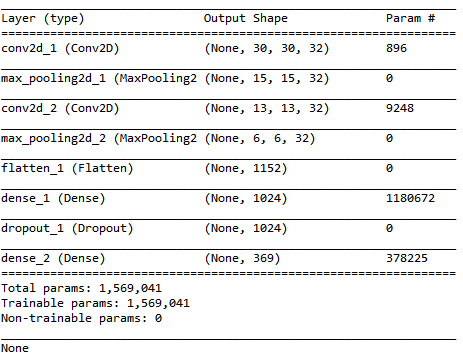
\includegraphics[width=4cm]{figures/1174008/7/praktik10.PNG}
            	\centering
           	 \caption{Praktik10}
       	 \end{figure}

\item Jelaskan kode program pada blok. Jelaskan arti dari setiap baris kode yang dibuat(harus beda dengan teman sekelas) dan hasil luarannya dari komputer sendiri.

Impor Modul Callbacks dari Librari Keras. Variabel callback mendefinisikan Callback ini untuk menulis log untuk TensorBoard, yang memungkinkan Anda untuk memvisualisasikan grafik dinamis dari pelatihan dan metrik pengujian Anda, serta histogram aktivasi untuk berbagai lapisan dalam model Anda.

\lstinputlisting[firstline=1, lastline=4]{src/1174008/7/11.py}

	\begin{figure}[H]
		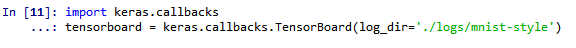
\includegraphics[width=4cm]{figures/1174008/7/praktik11.PNG}
            	\centering
           	 \caption{Praktik11}
       	 \end{figure}

\item Jelaskan kode program pada blok. Jelaskan arti dari setiap baris kode yang dibuat(harus beda dengan teman sekelas) dan hasil luarannya dari komputer sendiri.

Melakukan fit model dengan 32 ukuran subset dari sampel pelatihan Anda. Epoch sebanyak 10 kali. Vebrose=2 maksudnya menampilkan nomor dari epoch yang sedang berjalan atau yang sudah dijalankan. Validasi plit sebanayk 20\% sebagai fraksi data pelatihan untuk digunakan sebagai data validasi. Menggunakan TensorBoard sebagai callback untuk diterapkan selama pelatihan dan validasi. Variabel score mengembalikan nilai evaluate untuk menampilkan data lost dan data accuracy dari test. Menampilkan data loss dengan menghitung jumlah kemunculan nol. Menampilkan data accuracy dengan menghitung jumlah kemunculan 1.

\lstinputlisting[firstline=1, lastline=11]{src/1174008/7/12.py}

	\begin{figure}[H]
		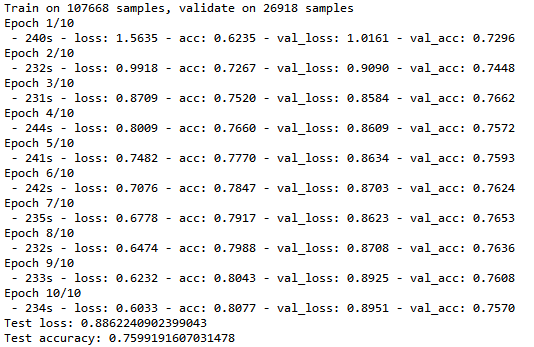
\includegraphics[width=4cm]{figures/1174008/7/praktik12.PNG}
            	\centering
           	 \caption{Praktik12}
       	 \end{figure}

\item Jelaskan kode program pada blok. Jelaskan arti dari setiap baris kode yang dibuat(harus beda dengan teman sekelas) dan hasil luarannya dari komputer sendiri.

Import modul time dari python anaconda. Variabel result berisikan array kosong. Menggunakan convolution 2D yang dimana akan memiliki 1 atau 2 layer. Mendefinisikan dense\_size dengan ukuran 128, 256, 512, 1024, 2048. Mendefinsikan drop\_out dengan 0, 25\%, 50\%, dan 75\%. Melakukan pemodelan Sequential. Jika ini adalah layer pertama, kita perlu memasukkan bentuk input. Kalau tidak kita hanya akan menambahkan layer. Kemudian, setelah menambahkan layer konvolusi, kita akan melakukan hal yang sama dengan max pooling. Lalu, kita akan meratakan atau flatten dan menambahkandense size ukuran apa pun yang berasal dari dense\_size. Dimana akan selalu menggunakan algoritma tanh. Jika dropout digunakan, kita akan menambahkan layer dropout. Menyebut dropout ini berarti, katakanlah 50\%, bahwa setiap kali ia memperbarui bobot setelah setiap batch, ada peluang 50\% untuk setiap bobot yang tidak akan diperbarui. Menempatkan ini di antara dua lapisan padat untuk dihidupkan dari melindunginya dari overfitting. Lapisan terakhir akan selalu menjadi jumlah kelas karena itu harus, dan menggunakan softmax. Itu dikompilasi dengan cara yang sama. Atur direktori log yang berbeda untuk TensorBoard sehingga dapat membedakan konfigurasi yang berbeda. Variabel start akan memanggil modul time atau waktu. Melakukan fit atau compile. MElakukan scoring dengan .evaluate yang akan menampilkan data loss dan accuracy dari model. end merupakan variabel untuk melihat waktu akhir pada saat pemodelan berhasil dilakukan. Menampilkan hasil dari run skrip diatas

\lstinputlisting[firstline=1, lastline=34]{src/1174008/7/13.py}

	\begin{figure}[H]
		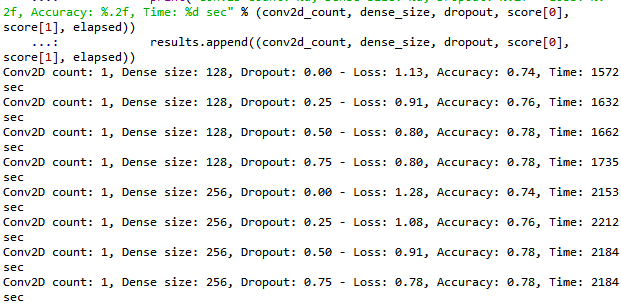
\includegraphics[width=4cm]{figures/1174008/7/praktik13.PNG}
            	\centering
           	 \caption{Praktik13}
       	 \end{figure}

\item Jelaskan kode program pada blok. Jelaskan arti dari setiap baris kode yang dibuat(harus beda dengan teman sekelas) dan hasil luarannya dari komputer sendiri.

Melakukan pemodelan Sequential. Untuk layer pertama, Menambahkan Convolutio 2D dengan dmensi 32, dan ukuran matriks 3x3 dengan function aktivasi yang digunakan yaitu relu dan menampilkan input\_shape. Dilakukan Max Pooling 2D dengan ukuran matriks 2x2. Untuk layer kedua, melakukan Convolusi lagi dengan kriteria yang sama tanpa menambahkan input, ini dilakukan untuk mendapatkan data yang terbaik. Flatten digubakan ntuk meratakan inputan. Menambahkan dense input sebanyak 128 neuron dengan menggunakan function aktivasi tanh. Dropout sebanyak 50\% untuk menghindari overfitting. Menambahkan dense pada model untuk output dimana layer ini akan menjadi jumlah dari class yang ada. Mengcompile model yang didefinisikan diatas. Menampilkan ringkasan dari pemodelan yang dilakukan

\lstinputlisting[firstline=1, lastline=12]{src/1174008/7/14.py}

	\begin{figure}[H]
		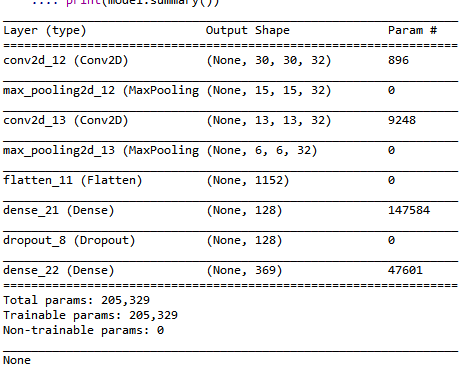
\includegraphics[width=4cm]{figures/1174008/7/praktik14.PNG}
            	\centering
           	 \caption{Praktik14}
       	 \end{figure}

\item Jelaskan kode program pada blok. Jelaskan arti dari setiap baris kode yang dibuat(harus beda dengan teman sekelas) dan hasil luarannya dari komputer sendiri.

Melakukan fit dengan join data train dan test agar dapat dilakukan pelatihan untuk jaringan pada semua data yang dimiliki.

\lstinputlisting[firstline=1, lastline=4]{src/1174008/7/15.py}

	\begin{figure}[H]
		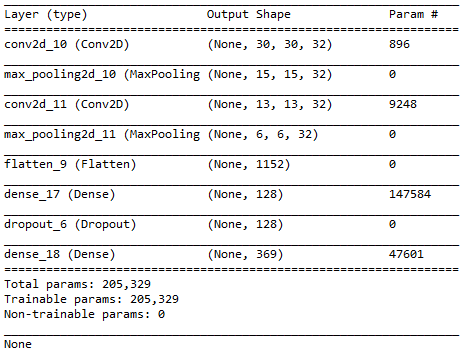
\includegraphics[width=4cm]{figures/1174008/7/praktik15.PNG}
            	\centering
           	 \caption{Praktik15}
       	 \end{figure}

\item Jelaskan kode program pada blok. Jelaskan arti dari setiap baris kode yang dibuat(harus beda dengan teman sekelas) dan hasil luarannya dari komputer sendiri.

Menyimpan atau save model yang telah di latih dengan nama mathsymbols.model.

\lstinputlisting[firstline=1, lastline=2]{src/1174008/7/16.py}

	\begin{figure}[H]
		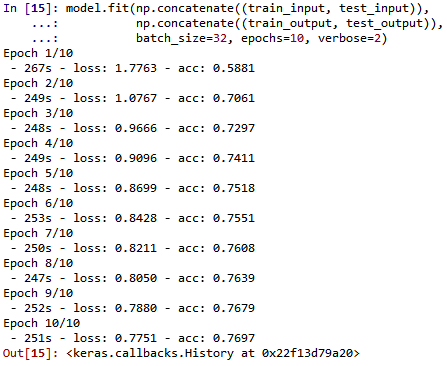
\includegraphics[width=4cm]{figures/1174008/7/praktik16.PNG}
            	\centering
           	 \caption{Praktik16}
       	 \end{figure}

\item Jelaskan kode program pada blok. Jelaskan arti dari setiap baris kode yang dibuat(harus beda dengan teman sekelas) dan hasil luarannya dari komputer sendiri.

Simpan label enkoder (untuk membalikkan one-hot encoder) dengan nama classes.npy

\lstinputlisting[firstline=1, lastline=2]{src/1174008/7/17.py}

	\begin{figure}[H]
		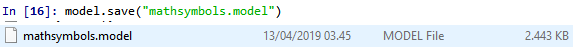
\includegraphics[width=4cm]{figures/1174008/7/praktik17.PNG}
            	\centering
           	 \caption{Praktik17}
       	 \end{figure}

\item Jelaskan kode program pada blok. Jelaskan arti dari setiap baris kode yang dibuat(harus beda dengan teman sekelas) dan hasil luarannya dari komputer sendiri.

Impor models dari librari Keras. Variabel model2 akan memanggil model yang telah disave.  Menampilkan ringkasan dari hasil pemodelan

\lstinputlisting[firstline=1, lastline=6]{src/1174008/7/18.py}

	\begin{figure}[H]
		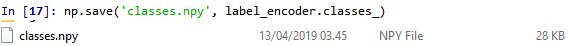
\includegraphics[width=4cm]{figures/1174008/7/praktik18.PNG}
            	\centering
           	 \caption{Praktik18}
       	 \end{figure}

\item Jelaskan kode program pada blok. Jelaskan arti dari setiap baris kode yang dibuat(harus beda dengan teman sekelas) dan hasil luarannya dari komputer sendiri.

Memanggil fungsi LabelEncoder. Variabel label\_encoder akan memanggil class yang disave sebelumnya. Function Predict akan mengubah gambar kedalam bentuk array. Variabel prediction akan melakukan prediksi untuk model2 dengan reshape variabel newimg dengan bentukarray 4D. Variabel inverted akan mencari nilai tertinggi output dari hasil prediks. Menampilkan hasil dari variabel prediction dan inverted

\lstinputlisting[firstline=1, lastline=14]{src/1174008/7/19.py}

	\begin{figure}[H]
		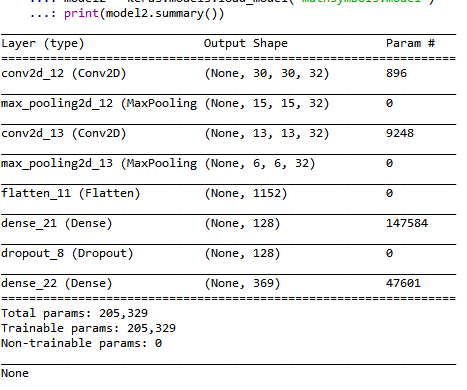
\includegraphics[width=4cm]{figures/1174008/7/praktik19.PNG}
            	\centering
           	 \caption{Praktik19}
       	 \end{figure}

\item Jelaskan kode program pada blok. Jelaskan arti dari setiap baris kode yang dibuat(harus beda dengan teman sekelas) dan hasil luarannya dari komputer sendiri.

Melakukan prediksi dari pelatihan dari gambar v2-00010.png. Melakukan prediksi dari pelatihan dari gambar v2-00500.png. Melakukan prediksi dari pelatihan dari gambar v2-00700.png

\lstinputlisting[firstline=1, lastline=6]{src/1174008/7/20.py}

	\begin{figure}[H]
		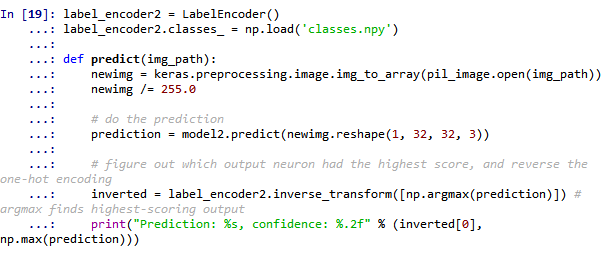
\includegraphics[width=4cm]{figures/1174008/7/praktik20.PNG}
            	\centering
           	 \caption{Praktik20}
       	 \end{figure}

\end{enumerate}

\subsection{Penanganan Error}
\begin{enumerate}

\item Berikut merupakan screenshot error
	\begin{figure}[H]
		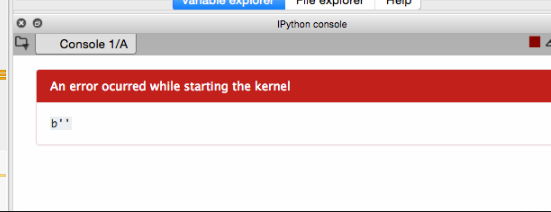
\includegraphics[width=4cm]{figures/1174008/7/error1.PNG}
            	\centering
           	 \caption{ERROR1}
       	 \end{figure}

\item Eror tersebut merupakan eror yang terjadi dan membuat kita tidak dapat mengakses dan menggunakan kernel atau konsol pada spyder.

\item Untuk penanganannya sebagai berikut :

Tutup spyder yang sedang dijalankan. Kemudian buka kembali spyder. Atau jika tidak berhasil, buka anaconda promt dan ketikan "conda update spyder". Jika tidak berhasil juga bisa menginstall ulang anaconda. Maka ketika dijaalankan lagi hasilnya seperti berikut 			\begin{figure}[H]
		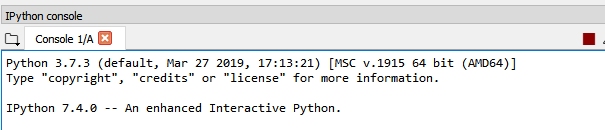
\includegraphics[width=4cm]{figures/1174008/7/error2.PNG}
            	\centering
           	 \caption{ERROR2}
       	 \end{figure}

\end{enumerate}

\subsection{Bukti Tidak Plagiat}
\begin{figure}[H]
\centering
	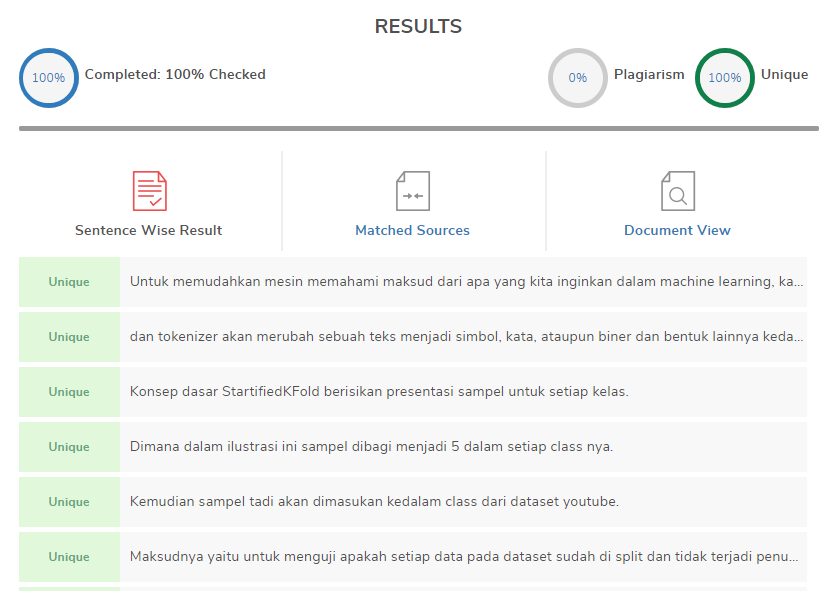
\includegraphics[width=4cm]{figures/1174008/7/bukticekplagiat.PNG}
	\caption{Bukti Tidak Melakukan Plagiat Chapter 7}
\end{figure}